\section{Query-Modulated Visual Processing Model}

Most models for tasks that resemble ours, such as VQA \parencite{Antol2015,Agrawal2016}, CLEVR \parencite{Johnson2017}  or Sort-of-CLEVR \parencite{Santoro}, tend to follow a similar form to the baseline model described above. First, we pass the image through a convolutional neural network, which processes it into some embedding (or latent representation) which the model can reason over. If the query is provided in natural language (as it is in VQA or CLEVR), it is independently processed to a separate embedding, almost always using a recurrent neural network. We then combine these two embeddings, of the question and of the image, and present the combined representation to another neural network, which attempts to compute the answer to the question on the image. A variety of different architectures have been proposed for these tasks, all broadly matching this description. These include several models examined by \textcite{Antol2015} in their work presenting the VQA paradigm, most models presented by \cite{Johnson2017} when introducing CLEVR, and the relational neural network discussed in \textcite{Santoro}. Several alternative models for these tasks propose defining and learning a set of individual ``modules,'' such ones to find particular objects or filter them based on relations, and learn both the weights for these modules as well as how to combine these modules to answer each query, building a unique computational graph for each different type of query \parencite{Johnson,Hu2017}. These models are substantially more powerful but correspondingly harder to implement and substantially more challenging to train.
\begin{figure}[!htb]
% \vspace{-0.225in}
\centering
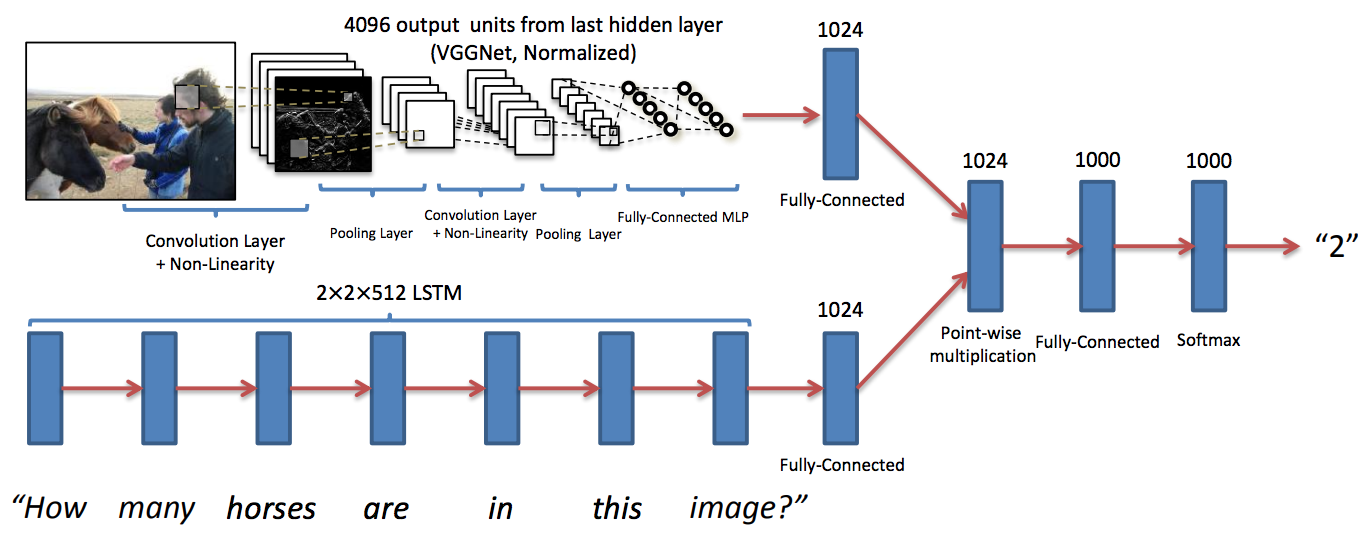
\includegraphics[width=\linewidth]{ch-models-compared/figures/reproduced.png}
\caption{{\bf VQA model diagram.} A schematic describing \possessivecite{Agrawal2016}'s best model, which independently processes the image and the question, combined the embeddings using element-wise multiplication, and feeds the combined embedding to a fully-conencted network to produce an answer. Reproduced from \textcite{Agrawal2016}.}
\label{fig:vqa-model-diagram}
% \vspace{-0.2in}
\end{figure}

We propose a model that strikes a middle ground between the two approaches described above, inspired by \textcite{Mozer2008}. In the first set of approaches, the image is processed into an embedding entirely independent of the query, which means that if we attempt to answer two separate questions on the same image, we will use the same visual embedding, only differing in the final, combined processing stage. On the other hand, we hoped to arrive at a model which does require the tremendous flexibility (and hence, complexity) of computing a different computational graph for each query. We found inspiration in the human visual system, where there is evidence for a tuning or modulation effect based on the task performed. \textcite{Cukur2013} use functional imaging to demonstrate that when subjects are asked to search movies for particular categories, such as `humans' or `vehicles,' their semantic representations shift to prioritize these categories, even when they do not exist in the stimuli presented. \textcite{Kay2015} and \textcite{Bracci2017} provide additional evidence for task-based and attentional modulation, impacting both the effectiveness of spatial coding and which properties of objects are represented. There is substantial recent research on how convolutional neural networks, on which our model is based, not only solve tasks well but also model activity in the human visual stream accurately \parencite{Yamins2016}. This line of work has produced a number of modifications to convolutional neural network architectures, which seek to augment these artificial models with additional features of the human visual system, such as recurrent and feedback connections \parencite{Spoerer2017,Nayebi2018} or different convolutional layers \parencite{Kubilius2018}. 

We offer a relatively uncomplicated approach which introduces the minimal augmentation to the baseline architecture that would enable query-based modulation. Recall that in the baseline model, the four convolutional layer groups included 16, 32, 48, and 64 filters respectively. In a convolutional architecture, each of these filters is passed over every spatial location in the input to that layer, computing a value for each location, which is then passed through an activation function (ReLU), batch-normalized, and pooled with adjacent values to be passed onto the next layer. To allow for query-based modulation, we introduce an additional layer, which maps from the query (a 30x1 vector) to the filters of a particular convolutional layer. The intuition is that different filters might be differentially relevant to distinguishing different properties of the input, and therefore being able to amplify or dampen the output of specific filters based on the query will help the model perform the task more effectively. This formulation allows us to achieve query-based modulation at miniscule additional computational cost, requiring only a single additional layer with under 2000 new parameters\footnote{The input (the query) is 30 units, and a bias unit is usually added. The maximal output size is 64, the number of filters in the last layers. Therefore, this layer requires $(30 + 1) \times 16 = 496$ weights to modulate the first convolutional layer, and $(30 + 1) \times 64 = 1984$ weights to modulate the last one.}. We compared each of the four possible depths of modulation, of augmenting each of the convolutional layer groups, as we did not know a priori which one (if at all) might produce results. Our approach is more naive than other modulation-based approaches, such as GaterNet \parencite{Chen}, who employ a secondary network to elect which filters to gate from a primary one, or FiLM \parencite{Perez2017,Dumoulin2018}, who employ a more complicated model architecture and interpret the modulation as conditioned normalization, an extension of batch normalization which normalizes based on the current input.   

In the context of our task and the sequential benchmark, we wish to examine a few questions. First, does introducing such query-based modulation improve the capacity to learn the baseline task (simultaneous, heterogeneous dimensions) -- that is, if we train a model on all thirty single-feature queries, using task-based modulation after the first, second, third, or fourth convolutional layer group, would it be able to learn the task faster. Second, if it improves performance with the entire dataset, will it behave similarly on the sequential benchmark? In other words, does it improve the capacity of the model to learn all queries simultaneously, or does it also improve the capacity to acquire the queries one at a time? Third, if it does improve performance on the sequential benchmark, does it demonstrate better scaling behavior? To elaborate this question, let us assume a query-modulated model indeed learns the queries faster when introduces in the sequential benchmark. Is it learning the initial queries more rapidly, but achieving similar performance on later ones? Is it learning all queries faster, but early queries equally faster as later ones? Alternatively, is it improving the scaling behavior, increasing the advantage over the baseline model as additional queries are introduced?